\title{NNPDF}
\author[Rosalyn Pearson]{}
\institute{University of Edinburgh}
\date{PDF4LHC}


\begin{frame}[fragile]{Deuteron and nuclear uncertainties}
We use an {\bf uncertainty} rather than a correcting the central value.
\newline
Theory covariance formalism previously developed in NNPDF.
      \begin{block}{Theory covariance matrix \tiny{ \textcolor{green}{[Ball, Nocera, Pearson: Eur.Phys.J.C 79 (2019) 3, 282 \& Eur.Phys.J.C 81 (2021) 1, 37]}}}
        \begin{equation}
            S_{ij} = \frac{1}{N_{rep}} \sum_k^{N_{rep}} \Delta_i^{(k)}\Delta_j^{(k)}
        \end{equation}
        \begin{equation}
            \Delta_i^{(k)} = T_i^{N}[f_{N}^{(k)}] - T_i^{N}[f_{p}]
        \end{equation}
      \end{block}
      
    \textbf{Deuteron:} NNLO deuteron PDFs fitted in NNPDF methodology 
    
    \textbf{Heavy nuclear:} NLO heavy nuclear PDFs from nNNPDF2.0 \tiny{ \textcolor{green}{[Abdul Khalek et al.: JHEP 09 (2020) 183]}}
  \begin{table}
    \caption{$\chi^2$ per deuteron/nuclear dataset}
        \resizebox{\linewidth}{!}{
    \begin{tabular}{rllllllll}
      \toprule
      Fit & {\bf Total} & BCDMS d & SLAC d & NMC p/d & E866/NuSea p/d & E605 Cu & NuTeV Fe & CHORUS Pb \\
      \midrule
      NNPDF4.0 & {\bf 1.174} & 1.015 & 0.4972 & 0.8194 & 0.3971 & 0.4907 & 0.4602 & 0.9372 \\
      No nuc unc & {\bf 1.265} & 1.313 & 0.8217 & 0.8167 & 0.8195 & 1.154 & 0.4569 & 1.165 \\
      \bottomrule
    \end{tabular}}
  \end{table}
\end{frame}

\begin{frame}{Per-point uncertainties}
\footnotesize{Deuteron (top) and heavy nuclear (bottom) }
\newline
\footnotesize{\textcolor{violet}{{\bf C:} experimental uncertainties}}
\newline
\footnotesize{\textcolor{orange}{{\bf S:} theory uncertainties (nuclear)}}
\newline
\footnotesize{\textcolor{cyan}{{\bf C+S:} total}}
  \begin{figure}
    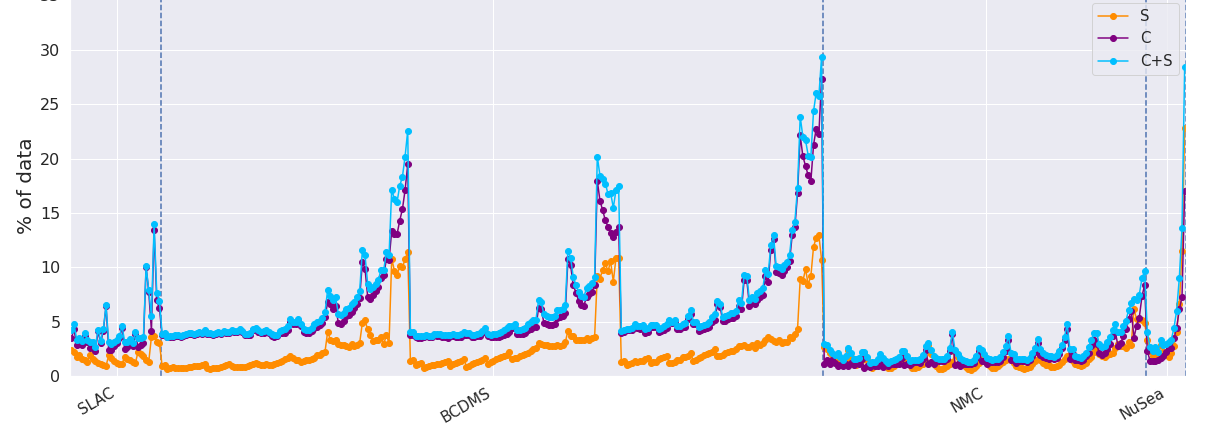
\includegraphics[width=85mm]{nuclear_uncs/diagdeut.png}
    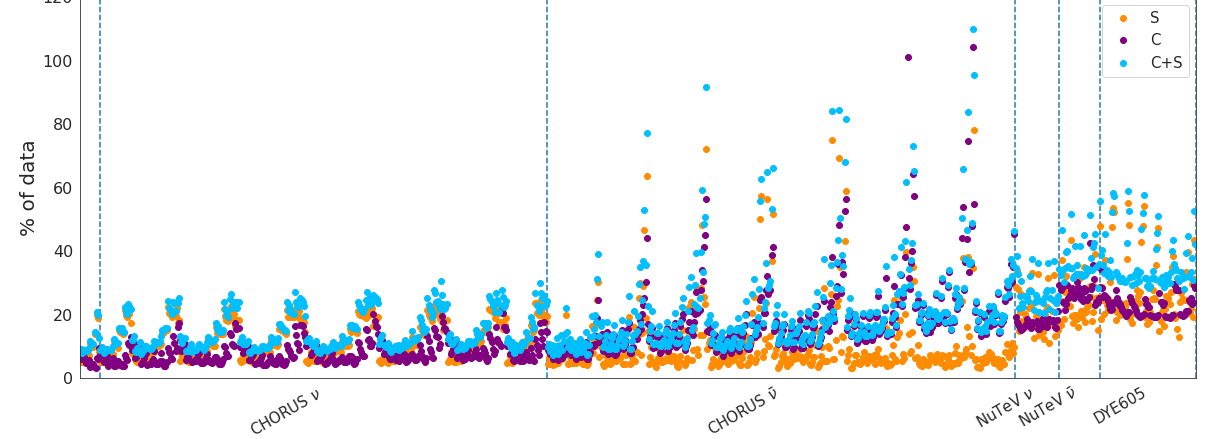
\includegraphics[width=85mm]{nuclear_uncs/diagnuc.png}
  \end{figure}
\end{frame}
